
\documentclass[%
 reprint,
%superscriptaddress,
%groupedaddress,
%unsortedaddress,
%runinaddress,
%frontmatterverbose, 
%preprint,
%preprintnumbers,
%nofootinbib,
%nobibnotes,
%bibnotes,
 amsmath,amssymb,
 aps,
%pra,
%prb,
%rmp,
%prstab,
%prstper,
%floatfix,
]{revtex4-2}
\usepackage{gensymb}
\usepackage{textcomp}
\usepackage{graphicx}% Include figure files
\usepackage{dcolumn}% Align table columns on decimal point
\usepackage{bm}% bold math
\usepackage{siunitx}
\usepackage{tabularx}
\usepackage{amssymb}
\usepackage{amsmath}
\usepackage{relsize}
\usepackage{caption}
\usepackage[colorlinks,bookmarks=false,citecolor=blue,linkcolor=blue,urlcolor=blue]{hyperref}
%\usepackage{hyperref}% add hypertext capabilities
%\usepackage[mathlines]{lineno}% Enable numbering of text and display math
%\linenumbers\relax % Commence numbering lines

%\usepackage[showframe,%Uncomment any one of the following lines to test 
%%scale=0.7, marginratio={1:1, 2:3}, ignoreall,% default settings
%%text={7in,10in},centering,
%%margin=1.5in,
%%total={6.5in,8.75in}, top=1.2in, left=0.9in, includefoot,
%%height=10in,a5paper,hmargin={3cm,0.8in},
%]{geometry}

\begin{document}

\preprint{APS/123-QED}

\title{The Franck-Hertz Experiment}% Force line breaks with \\


\author{Maitrey Sharma}
\email{maitrey.sharma@niser.ac.in}
\affiliation{School of Physical Sciences, National Institute of Science Education and Research, HBNI, Jatni-752050, India}




\date{\today}% It is always \today, today,
             %  but any date may be explicitly specified

\begin{abstract}
In this experiment, we study the Franck-Hertz experiment using Ne and Hg tubes, and eventually calculate \textbf{the excitation energy} and \textbf{the mean free path} of a bombarded electron in a Hg gas tube setup at $175 ^{\circ} C$ and $190 ^{\circ} C$, respectively. The Franck-Hertz experiment essentially establishes that the energy levels of an atom are \textit{\textbf{quantized}}. It is seen that when the Ne or Hg atoms in a gas tube are bombarded with charged particles (electrons), a distinct number energy minima of the of electrons is seen (resulting due to inelastic collisions), indicating that the atoms only absorb (and release) only specific energy values to get excited (and return to ground state). This experiment is considered quite important for modern quantum mechanical picture of an atom, mainly because it experimentally supported Bohr's atomic model.
\end{abstract}

\keywords{Topological Hall Effect}
\maketitle

%\tableofcontents

\section{\label{sec:level1}Introduction}
    In the summer of 1913, Niels Bohr published a model for atoms that turned out be quite successful in accounting for the optical properties of atomic hydrogen. It introduced the concept of quantized energy states and further solidified the foundations of quantum mechanics. But it was the series of the experiments published by James Franck and Gustav Hertz in the following year which first clearly showed the quantum nature of atoms. Since then, the Franck-Hertz experiment on electron-mercury collisions is one of the key demonstrations of the quantum behavior of atoms and provides a direct non-optical demonstration of the existence of discrete stationary energy levels in atoms. Usually the experiment is limited to the determination of the energy required to excite the first energy levels of mercury or neon atoms.
    \par
    
    In the original experiments published in the spring of 1914 over several months, Franck and Hertz discovered that electrons moving through the Hg vapour with an energy equal to or greater than a certain critical value ($\SI{4.9}{\electronvolt}$) can excite the $\SI{253.6}{\nm}$ line of Hg. Electrons with less than the critical merely bounce off elastically when they collide with Hg atom and fail to excite any electromagnetic radiation at all. And thus, this experiment provided crucial crucial evidence in favor of Bohr Theory. In this experiment, we will accelerate electrons in both Hg as well as Ne tubes.
    

\section{Experimental Setup}
    The Franck-Hertz tube is a tetrode (see figures (\ref{fig:tetrodeUp1}) and (\ref{fig:tetrodeUp2})) with an indirectly heated barium oxide cathode $K$, a mesh-type control grid $G$, a mesh-type anode $A$, and a collector electrode $E$ (see figure (\ref{fig:wide})). $U_F$ represents the filament voltage, $U_A$ the accelerating voltage, $U_{AE}$ the counter voltage and $U_{KG}$ is the control voltage. The electrodes are in a plane-parallel configuration. The distance between the control grid and the anode grid is about $\SI{5}{\milli \metre}$, and the distances between the cathode and the control grid and between the anode and the collector electrode are both about $\SI{2}{\milli \metre}$. The tube is supplied already filled with neon gas at a pressure chosen to give an optimum characteristic curve, which is in the region of several hundred Pascal.
    \begin{figure}
        \centering
        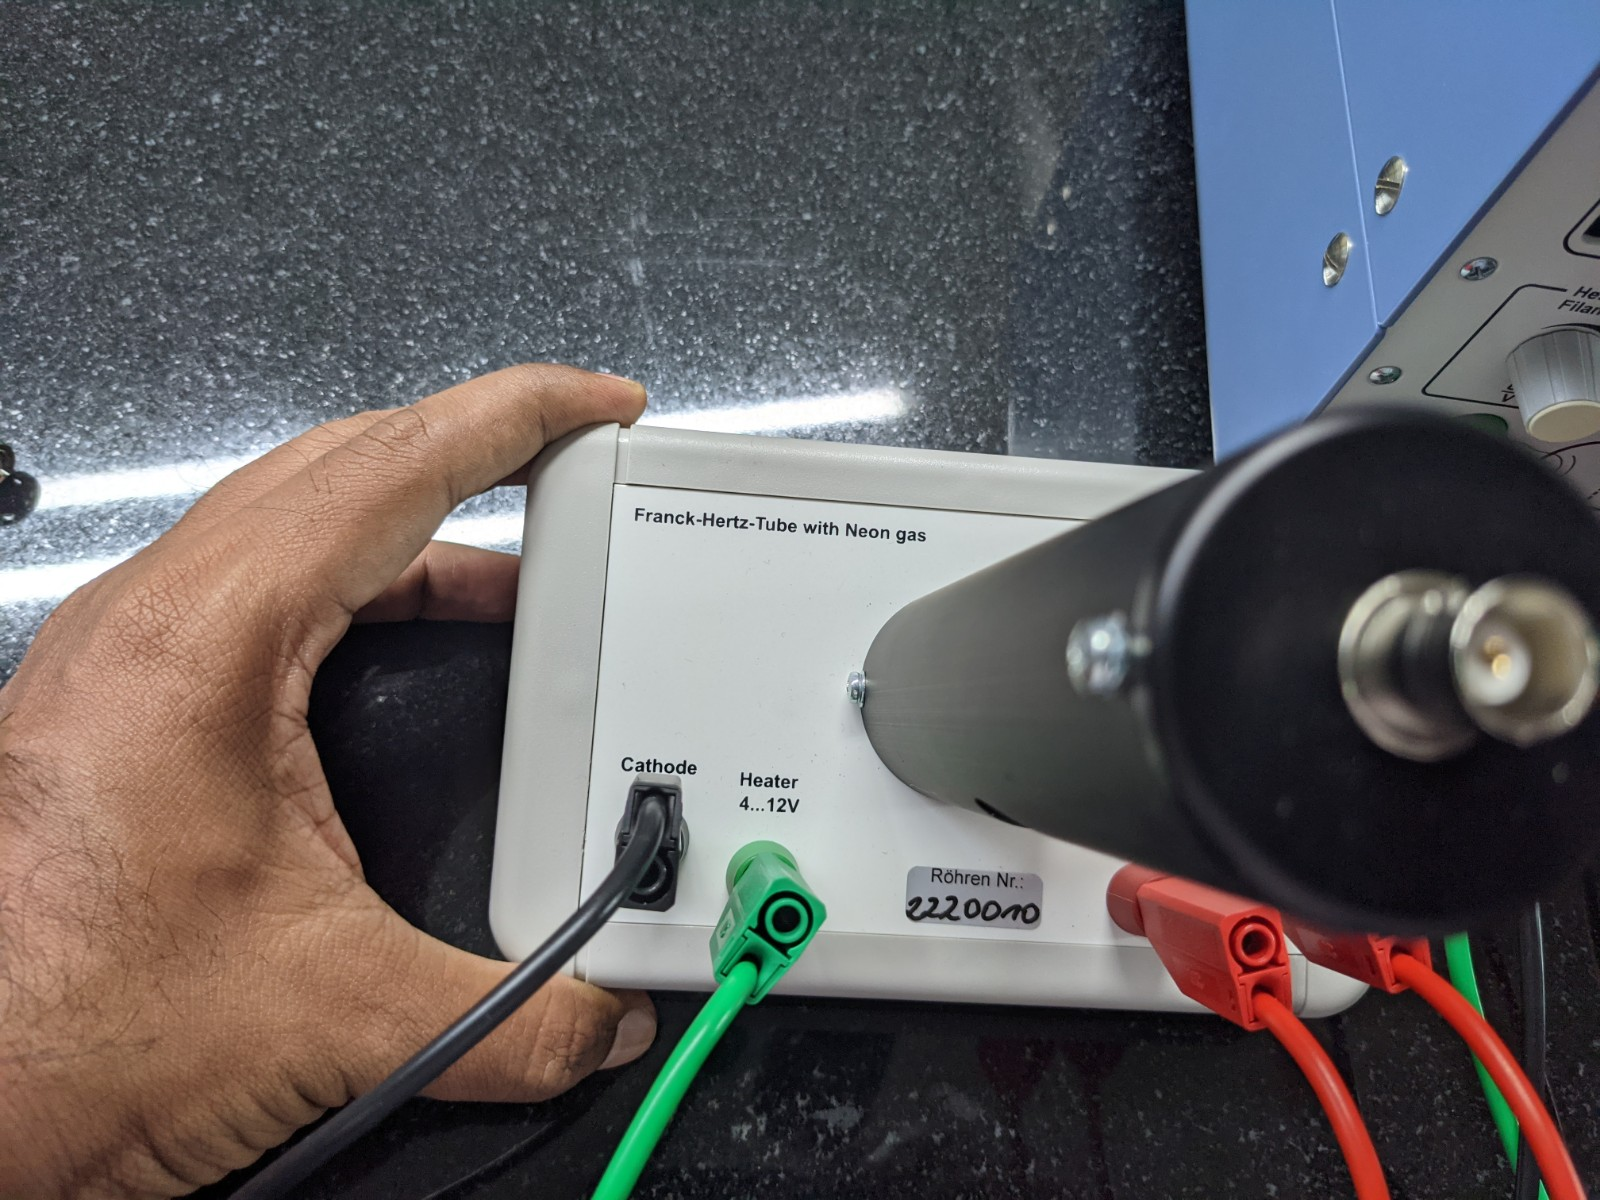
\includegraphics[scale = 0.12]{Figures/tetrodeup1.jpg}
        \caption{The tetrode setup from top left.}
        \label{fig:tetrodeUp1}
    \end{figure}
    \begin{figure}
        \centering
        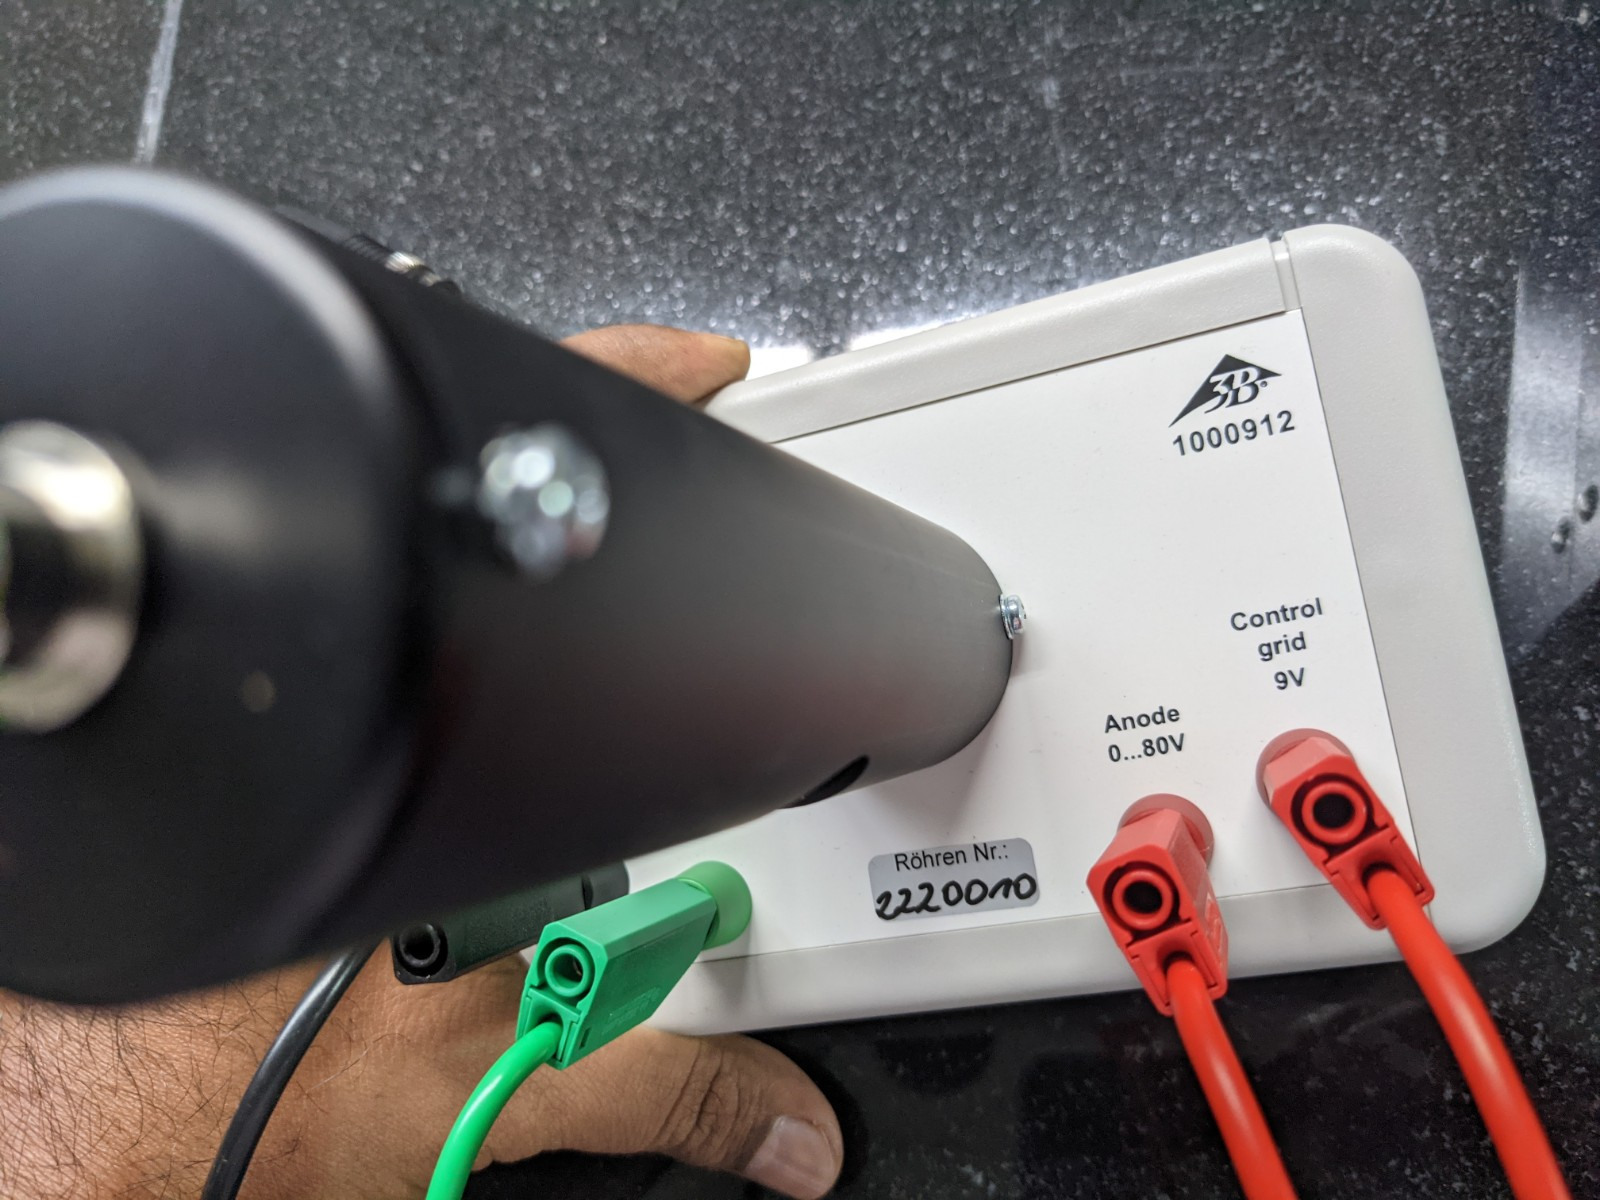
\includegraphics[scale = 0.12]{Figures/tetrodeup2.jpg}
        \caption{The tetrode setup from top right.}
        \label{fig:tetrodeUp2}
    \end{figure}
    \begin{figure*}
    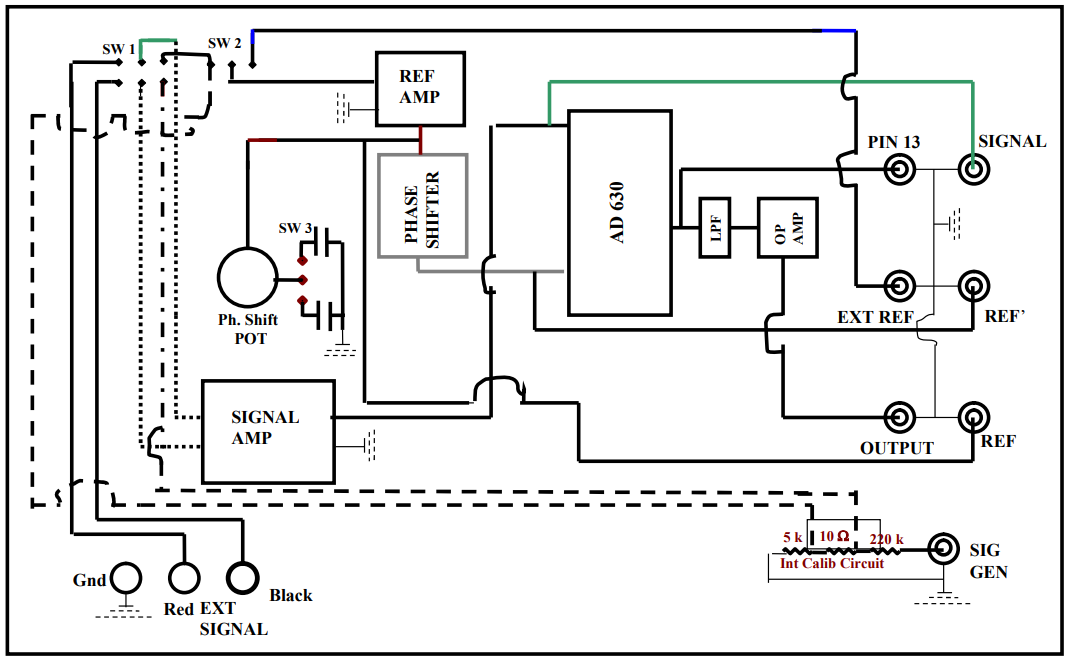
\includegraphics[scale = 0.5]{Figures/schematic.png}
    \caption{\label{fig:wide}Schematic of set up for measuring the Franck-Hertz curve for Neon}
    \end{figure*}
    \par
    The connecting sockets for the heater, control grid and anode grid voltages are on the base of the instrument. The collector current is taken off through the $BNC$ socket at the top end of the screening cylinder. An internal $\SI{10}{\kilo \ohm}$ limiting resistor is permanently built in between the connector sockets for the accelerator (control grid) voltage and the anode voltage. This protects the tube in case there is a spark discharge caused by applying too high a voltage. The voltage loss in this resistor when making measurements is negligible, as the anode current in the tube is smaller than $\SI{5}{\pico \ampere}$. (Thus the voltage loss in the protecting resistor is $\SI{0.05}{\volt}$.)

\section{Theory}
    Neon atoms are excited by inelastic collision with electrons emitted by the cathode in a Frank-Hertz tube. The cathode in the tube is heated by a filament to emit electrons in a process called thermionic emission. After absorbing energy from collisions, electrons in Ne atoms are excited and subsequently de-excited to produce a visible glow in the gas that can be viewed directly. The energy level diagram for Ne is shown in figure (\ref{fig:energyLevelNe}) and (\ref{fig:energyLevelNe2}).
    \begin{figure}[b]
        \centering
        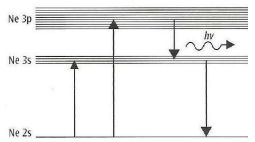
\includegraphics{Figures/neonstates.png}
        \caption{Energy Level Diagram for Ne}
        \label{fig:energyLevelNe}
    \end{figure}
    \begin{figure}
        \centering
        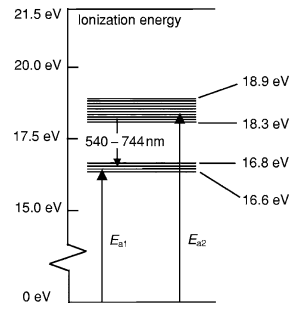
\includegraphics{Figures/neonstates2.png}
        \caption{Selected energy levels for Ne\cite{Moore}}
        \label{fig:energyLevelNe2}
    \end{figure}
    The most probable excitation through inelastic electron collision takes place from the ground state to the ten 3$p$-states, which are between $\SI{18.4}{\electronvolt}$ and $\SI{19.0}{\electronvolt}$ above the ground state. The four lower 3$s$-states in the range from $\SI{16.6}{\electronvolt}$ and $\SI{16.9}{\electronvolt}$ are excited with a lower probability. The de-excitation of the 3$p$ states to the ground is only possible via the 3$s$-states. The 3$p$-3$s$ transition leads to emission of a photon. The light emitted in this process lies in the visible range between red and green, and can thus be observed with the naked eye.
    \begin{figure}
        \centering
        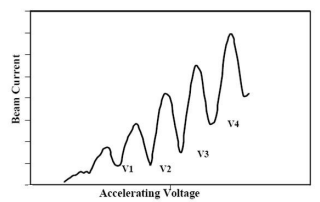
\includegraphics{Figures/typicalcurve.png}
        \caption{Typical Franck-Hertz curve showing plate current versus accelerating voltage characteristics.}
        \label{fig:typical1}
    \end{figure}
    \par
    In the Franck-Hertz tube, electrons are emitted from the cathode and form a charge cloud. These electrons are accelerated by the accelerating voltage $U_A$ between the cathode $K$ and anode $A$. A braking voltage $U_{AE}$ is present between anode $A$ and collector electrode $E$. Only electrons with sufficient kinetic energy can reach the electrode $E$ and contribute to the collector current. A typical curve is shown in figure (\ref{fig:typical1}) and for Hg in figure (\ref{fig:typicalHg}).
    \begin{figure}
        \centering
        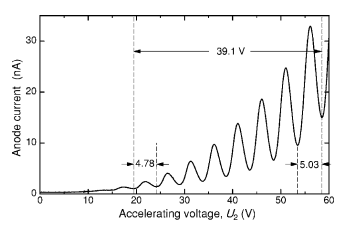
\includegraphics[scale = 0.9]{Figures/typicalhg.png}
        \caption{Typical Franck-Hertz curve recorded with Hg tube at 170 \degree C.}
        \label{fig:typicalHg}
    \end{figure}
    \par
    As the acceleration voltage $U_A$ is increased while $U_F$, $U_{KG}$ and $U_{AE}$ are held constant, the corresponding collector current initially increases and reaches a maximum when the kinetic energy of the electrons closely in front of anode $A$ is just sufficient to transfer the energy required to excite the neon atoms through collisions. The collector current drops off dramatically, as after collision the electrons can no longer overcome the braking voltage $U_{AE}$. As the acceleration voltage $U_A$ increases, the electrons attain the energy level required for exciting the neon atoms at ever greater distances from anode $A$. After collision, they are accelerated once more and, when the acceleration voltage is sufficient, again absorb so much energy from the electrical field that they can excite a neon atom. The result is a second maximum, and at greater voltages $U_A$ further maxima of the collector currents are observed. At higher acceleration voltages, we can observe discrete red luminance layers between grid $G$ and anode $A$ as shown in figure (\ref{fig:layers}).
    \begin{figure}[h]
        \centering
        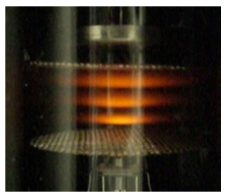
\includegraphics{Figures/layers.png}
        \caption{Visible luminescence layers between grids.}
        \label{fig:layers}
    \end{figure}
    \par
    The energy required to transfer an electron from ground state to an excited state (or a state of higher energy) is called \textbf{excitation energy} of the electron in that state. It is generally assumed that all the maxima or minima spacings in Franck-Hertz curves are equal and correspond to the first excitation energy of atoms. It is even suggested that the magnitude of the lowest excitation energy can be calculated by using the mean value of the maxima or minima spacings.
    \begin{figure}
        \centering
        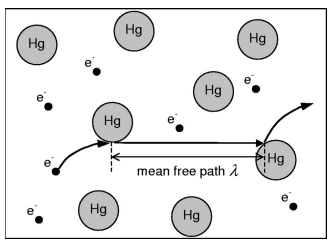
\includegraphics[scale = 0.9]{Figures/meanfree.png}
        \caption{Schematic of the energy transfer from electrons to atoms.}
        \label{fig:meanFreePath}
    \end{figure}
    \par
    Figure (\ref{fig:meanFreePath}) shows the motion of an electron between two grids in a Hg tube in the presence of the accelerating potential $U_A$. While it accelerates the electron gains energy and collides with mercury atoms. If the electron energy is smaller than the lowest excitation energy of the mercury atoms, the collisions are elastic and the energy loss by the electron is very small because of the large mass difference between the colliding particles. If the electron energy reaches the excitation threshold of Hg atoms, inelastic collisions may occur. Before the inelastic collision takes place, an electron must come close to a mercury atom.The average distance that an electron moves before the inelastic collision takes place is the \textbf{mean free path} $\lambda$.
    \par
    Figure (\ref{fig:gridLevels}(a)) shows the energy gain of a free electron moving in the tube between the two grids. Figure (\ref{fig:gridLevels}(b)) illustrates how an electron gains energy at a higher accelerating potential in comparison to figure (\ref{fig:gridLevels}(a)). 
    \begin{figure}[b]
        \centering
        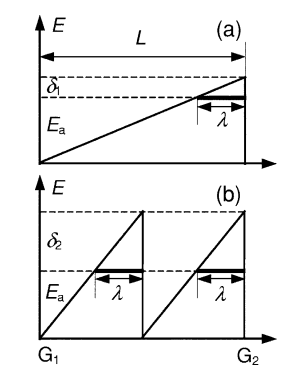
\includegraphics{Figures/gridlevels.png}
        \caption{Electron energy between grids $G_1$ and $G_2$ in a Franck-Hertz tube with an accelerating voltage sufficient for one (a) and two (b) inelastic collisions. $E_a$ is the lowest excitation energy of atoms, and $\delta_1$ and $\delta_2$ are additional energies gained by the electrons along the mean free path $\lambda$.}
        \label{fig:gridLevels}
    \end{figure}
    \par
    For n inelastic collisions the energy gained by the electrons is \cite{2006AmJPh..74..423R}
    \begin{equation}
    \label{eq1}
        E_n = n(E_a + \delta_n)
    \end{equation}
    At typical tube pressures, the mean free path of the electrons is much less than the distance between two grids, $\lambda \ll L$. With this assumption we have $\delta_n \ll E_a$ and
    \begin{equation}
    \label{eq2}
        \delta_n = n \frac{\lambda}{L} E_a
    \end{equation}
    Using (\ref{eq1}) and (\ref{eq2}), we can deduce that the spacing between two minimas ($\Delta U_A$) in a Franck-Hertz curve increases linearly with the minimum order $n$, and
    \begin{equation}
    \label{eq3}
        \boxed{E_a = \Delta U_A(0.5)}
    \end{equation}
    The equation for $\Delta U_A$ can be found by the linear fit of the $\Delta U_A \sim n$ plot.
    The mean free path can also be derives using (\ref{eq1}) and (\ref{eq2}) as
    \begin{equation}
    \label{eq4}
        \boxed{\lambda = \frac{L}{2 E_a} \frac{d \Delta U(n)}{dn}}
    \end{equation}
    That is, the second term denotes the slope of the $\Delta U_A \sim n$ plot.
    
\section{Experimental Procedure}
    \begin{enumerate}
        \item We begin by putting the selector switch in the manual mode. (The operating unit for the experiment is shown in figures (\ref{fig:HgSetup}) and (\ref{fig:NeSetup})).
        \item All the control knobs are set at extreme anticlockwise position of the Franck Hertz base unit.
        \item The Franck Hertz operating unit is connected to mains via a plug and the unit is switched ON.
        \item The filament or the heater voltage $U_F$ is gradually increased till the filament starts glowing. We approximate the filament voltage, $U_F$ to be around $\SI{8}{\volt}$ or $\SI{9}{\volt}$ and then process to wait for 3-5 minutes.
        \item The control voltage $U_{KG}$ is set around $\SI{4}{\volt}$ to $\SI{6}{\volt}$ and the counter voltage $U_{AE}$ is set around $\SI{4}{\volt}$ to $\SI{8}{\volt}$ approximately.
        \item We keep the $U_F$, $U_{KG}$ and $U_{AE}$ fixed, and start slowly varying the acceleration voltage $U_A$ from $\SI{0}{\volt}$ to $\SI{80}{\volt}$ and record the corresponding collector current.\\
        \textbf{Note: } Sometimes due to double and multiple collisions of electrons and combinations of excitation of 3$s$ level and 3$p$ level, there may be small variations in plate current measured in nanoampere. In such cases, we take the mean of minimum and maximum readings keeping $U_A$ constant.
        \item The experiment is repeated for different filament voltages $U_F$ and $U_{KG}$. We may adjust the counter voltage $U_{AE}$, if required.
        \item For Ne, the minimas and maximas are not as well defined so we will skip the rigorous analysis of it. Just recording their values is enough.
        \item We repeat all steps for Hg tube similarly at 175\degree C and 190\degree C, respectively.
        \item Finally, we analyse the curve to obtain explicit values of the maxima and minima of the curve, which will help in calculating the excitation energy and the mean free path.
        \item For the analysis part, we plot the $I_A \sim U_A$ curve and record the minimas in order to obtain the minima spacings, that is, $\Delta U_A$.
    \begin{figure}
        \centering
        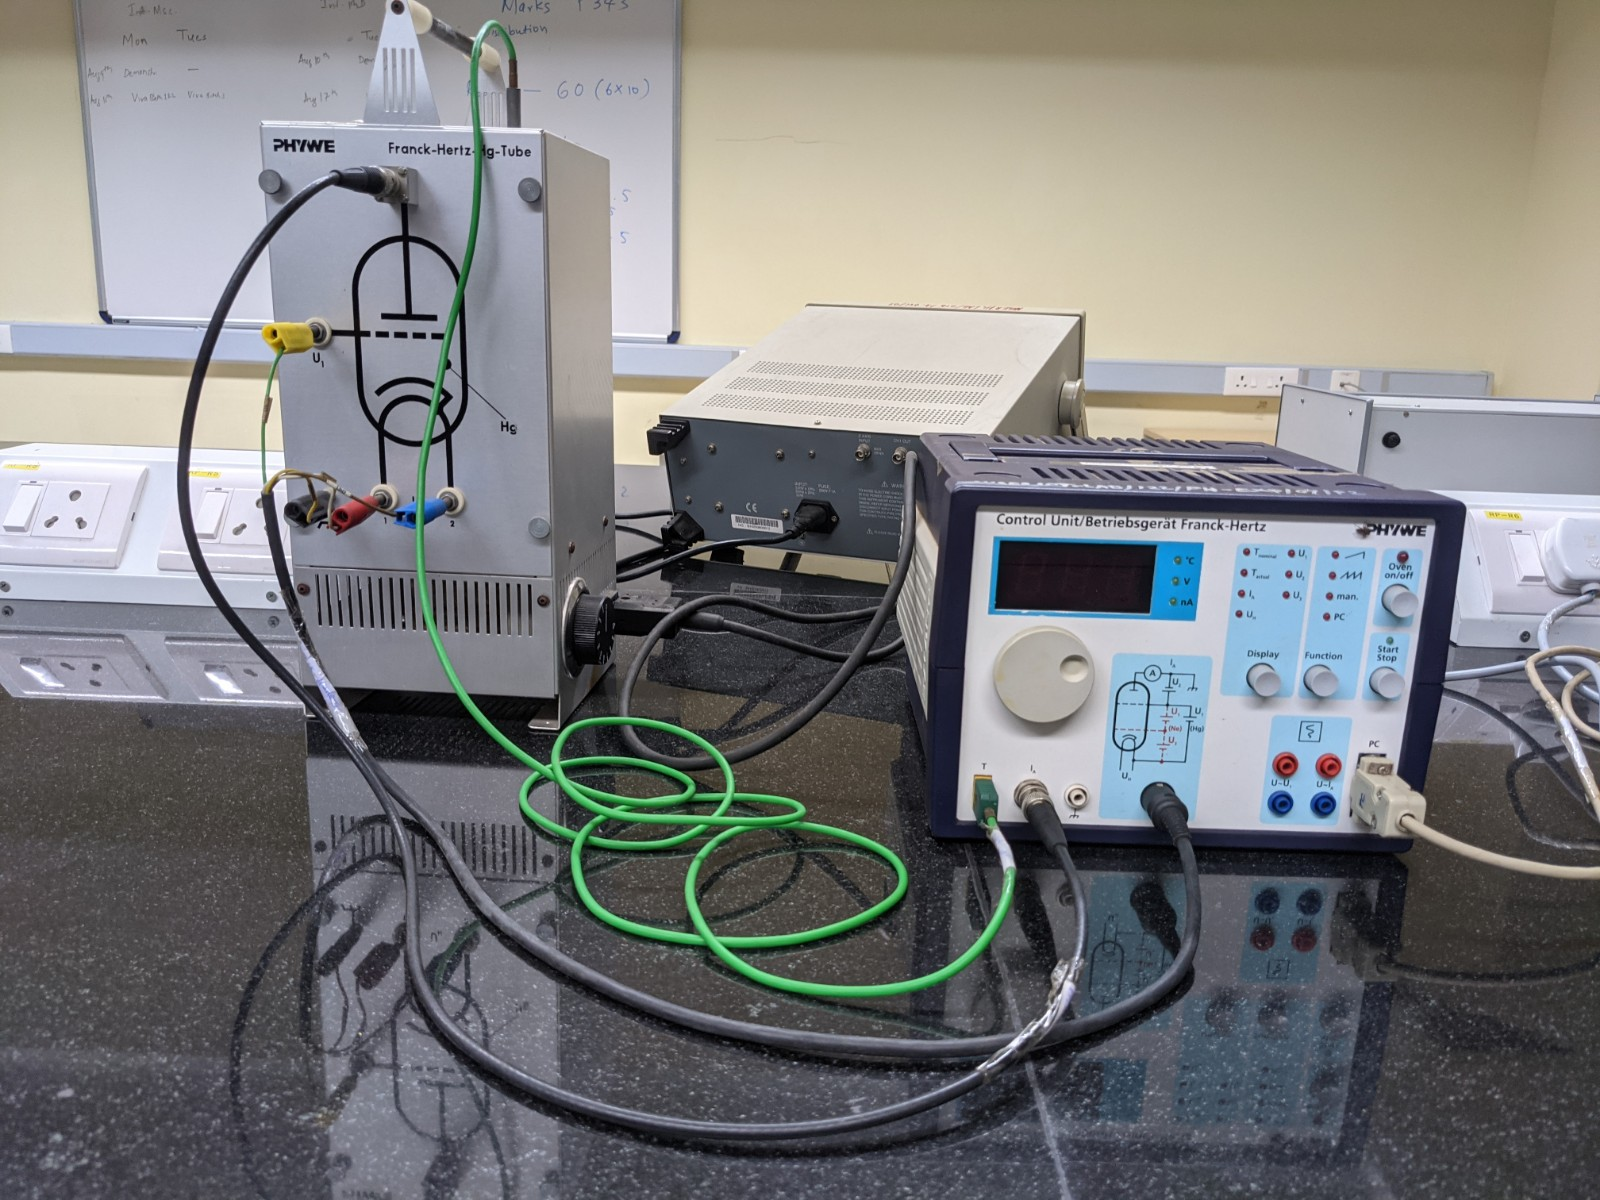
\includegraphics[scale = 0.12]{Figures/hgsetup.jpg}
        \caption{The Franck-Hertz operating unit in Hg setup.}
        \label{fig:HgSetup}
    \end{figure}
    \begin{figure}
        \centering
        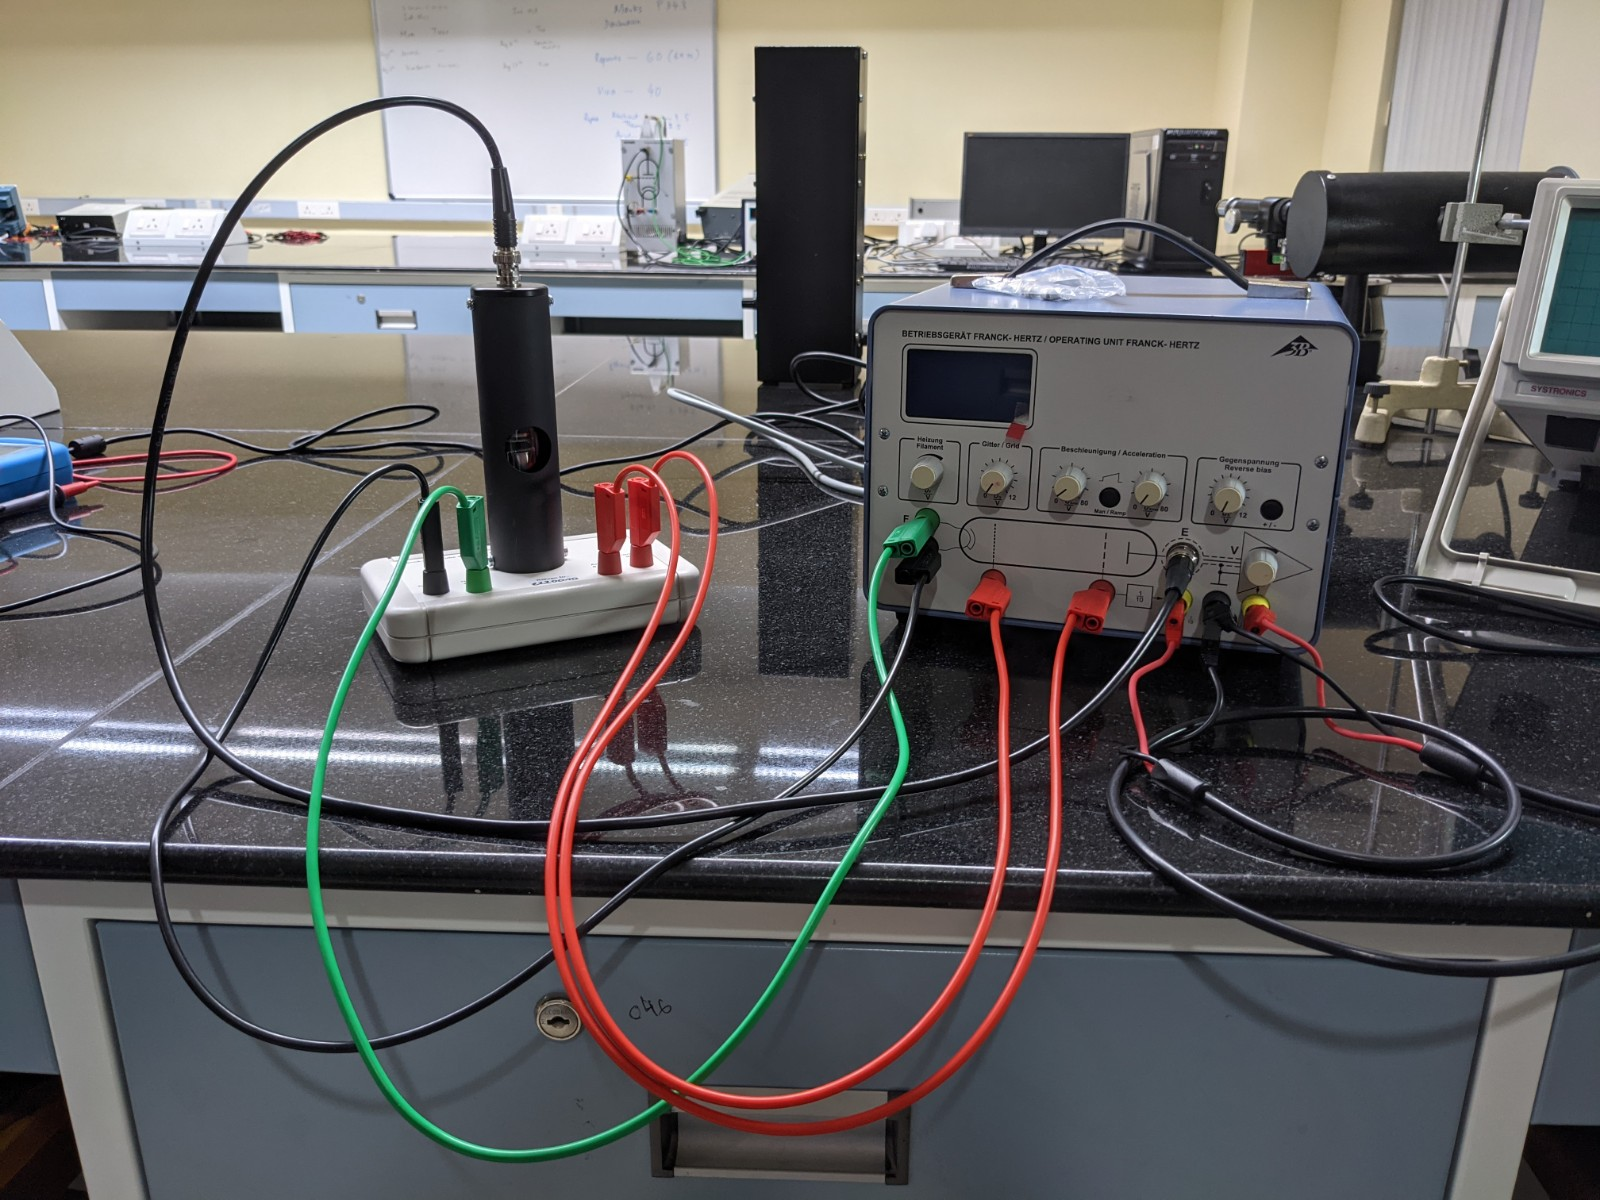
\includegraphics[scale = 0.12]{Figures/nesetup.jpg}
        \caption{The Franck-Hertz operating unit in Ne setup}
        \label{fig:NeSetup}
    \end{figure}
    \end{enumerate}
    
    
\section{Observations}
    The make of the Ne tube setup is 3B Scientific and that of Hg tube is Phywe. The following parameters are recorded before taking the observations.
    \begin{enumerate}
        \item For the Ne tube the set parameters are as follows: filament voltage $U_F = \SI{8.5}{\volt}$, counter voltage $U_{AE} = \SI{5.3}{\volt}$ and control voltage, $U_{KG} = \SI{4.5}{\volt}$.
        \item The length of the Ne tube is $L = \SI{5}{\milli \metre}$.
        \item The length of the Hg tube is $L = \SI{7}{\milli \metre}$.
        \item The accelerating voltage $U_A$ is set to $\SI{80}{\volt}$.
    \end{enumerate}
    In case of a Neon tube, three distinct orange-red rings are observed one after another on increasing the accelerating voltage $U_A$ slowly, and after increasing over a certain limit, the rings converge. The distinct rings seen are actually indicative of the excitation of Ne atoms from the ground to 3$p$ state, which emits light in the visible range. The three separate rings correspond to the three \textbf{dips} in collector current, which is later seen in figure (\ref{fig:neonPlot}), and this process is observed to repeat thereafter.
    \par
    The following are the plots for Ne tube and the Hg tubes at 175\degree C (figure (\ref{fig:175Hg})) and 190\degree C (figure (\ref{fig:190Hg})).
    \begin{figure}[htp]
        \centering
        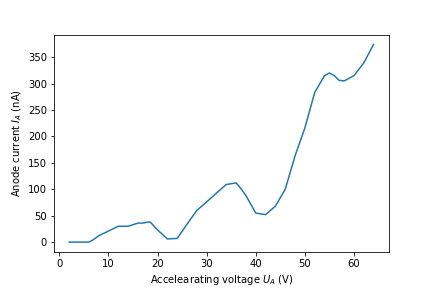
\includegraphics[scale = 0.5]{Figures/NeonPlot.png}
        \caption{Experimentally obtained Franck-Hertz curve for Neon tube.}
        \label{fig:neonPlot}
    \end{figure}
    \begin{figure}[htp]
        \centering
        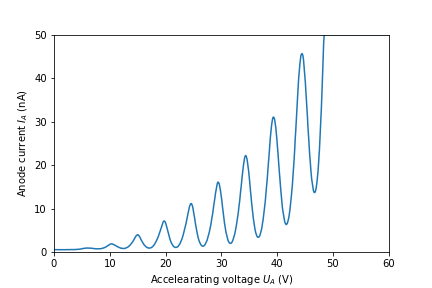
\includegraphics[scale = 0.5]{Figures/175HgPlot.png}
        \caption{Experimentally obtained Franck-Hertz curve for Mercury tube at 175\degree C.}
        \label{fig:175Hg}
    \end{figure}
    \begin{figure}[htp]
        \centering
        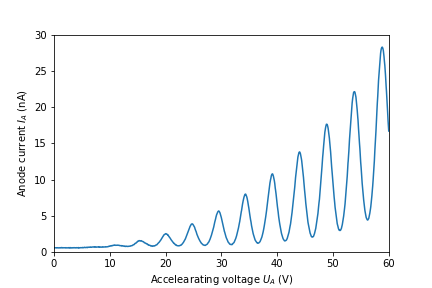
\includegraphics[scale = 0.5]{Figures/190HgPlot.png}
        \caption{Experimentally obtained Franck-Hertz curve for Mercury tube at 190\degree C.}
        \label{fig:190Hg}
    \end{figure}

\section{Results and discussions}
    From the plots obtained we can deduce some important results through which we will find our required values of excitation energy and mean free path.
    \subsection{Neon Tube}
        As the resolution of the data obtained from the experiment using the Neon tube is not good, the rigorous analysis employing the use of minima spacings is not feasible. So, we will just enumerate the maximas and minimas obtained. 
        \begin{enumerate}
            \item The first maxima: ($\SI{18.5}{\volt}$, $\SI{38}{\nano \ampere}$)
            \item The first minima: ($\SI{22}{\volt}$, $\SI{6}{\nano \ampere}$)
            \item The second maxima: ($\SI{36}{\volt}$, $\SI{112}{\nano \ampere}$)
            \item The second minima: ($\SI{42}{\volt}$, $\SI{52}{\nano \ampere}$)
            \item The third maxima: ($\SI{55}{\volt}$, $\SI{320}{\nano \ampere}$)
            \item The third minima: ($\SI{58}{\volt}$, $\SI{305}{\nano \ampere}$)
        \end{enumerate}
        From here, using the 2 minima spacings and (\ref{eq3}), we can conclude that the excitation energy for Ne will be \boxed{$E_a = \SI{22}{\electronvolt}$}.
    \subsection{Mercury Tube}
        The resolution of the data obtained from the experiment using mercury is satisfactory enough to do further analysis.
        \subsubsection{At 175\degree C}
            The voltages for which minimas were obtained for the experiment done at 175 \degree C using the Hg tube are: $\SI{17.16}{\volt}$, $\SI{21.9}{\volt}$, $\SI{26.81}{\volt}$, $\SI{31.77}{\volt}$, $\SI{36.67}{\volt}$, $\SI{41.68}{\volt}$, and $\SI{46.71}{\volt}$.
            From this, we can tabulate $\Delta U_A$. The resulting linear fit is plotted as figure (\ref{fig:175HgMS}). 
            \begin{table}[h!]
            \caption{Minima spacings at 175\degree C}
            \begin{tabular}{|m{1cm}|m{2cm}|}
            \hline
            \hfil $\bm{n}$ & \hfil $\bm{\Delta U_A}$ \\ \hline \hline
            \hfil 2 & \hfil 4.74 \\ \hline
            \hfil 3 & \hfil 4.91 \\ \hline
            \hfil 4 & \hfil 4.96 \\ \hline
            \hfil 5 & \hfil 4.90 \\ \hline
            \hfil 6 & \hfil 5.01 \\ \hline
            \hfil 7 & \hfil 5.03 \\ \hline
            \end{tabular}
            \label{Tab:175Hg}
            \end{table}
            \begin{figure}[]
                \centering
                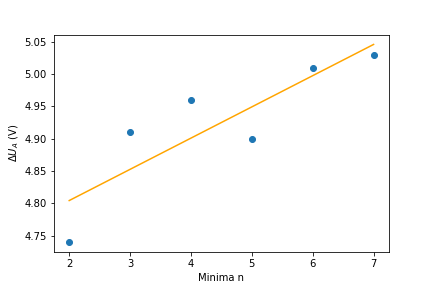
\includegraphics[scale = 0.5]{Figures/175HgMS.png}
                \caption{$\Delta U_A \sim n$ for Hg tube at 175\degree C.}
                \label{fig:175HgMS}
            \end{figure}
        \subsubsection{At 190\degree C}
            The voltages for which minimas were obtained for the experiment done at 190\degree C using the Hg tube are: $\SI{22.49}{\volt}$, $\SI{27.2}{\volt}$, $\SI{31.94}{\volt}$, $\SI{36.67}{\volt}$, $\SI{41.46}{\volt}$, $\SI{46.39}{\volt}$, $\SI{51.3}{\volt}$ and $\SI{56.23}{\volt}$. From this, we can tabulate $\Delta U_A$. The resulting linear fit is plotted as figure (\ref{fig:190HgMS}).
            \begin{table}[h!]
            \caption{Minima spacings at 190\degree C}
            \begin{tabular}{|m{1cm}|m{2cm}|}
            \hline
            \hfil $\bm{n}$ & \hfil $\bm{\Delta U_A}$ \\ \hline \hline
            \hfil 2 & \hfil 4.71 \\ \hline
            \hfil 3 & \hfil 4.74 \\ \hline
            \hfil 4 & \hfil 4.73 \\ \hline
            \hfil 5 & \hfil 4.79 \\ \hline
            \hfil 6 & \hfil 4.93 \\ \hline
            \hfil 7 & \hfil 4.91 \\ \hline
            \hfil 8 & \hfil 4.93 \\ \hline
            \end{tabular}
            \label{Tab:190Hg}
            \end{table}
            \begin{figure}[]
                \centering
                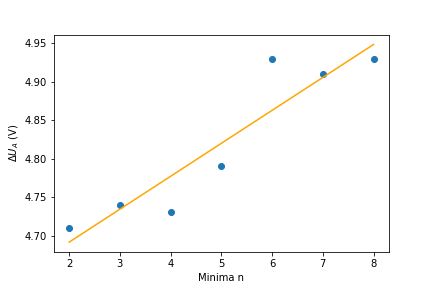
\includegraphics[scale = 0.5]{Figures/190HgMS.png}
                \caption{$\Delta U_A \sim n$ for Hg tube at 190\degree C.}
                \label{fig:190HgMS}
            \end{figure}
\section{Calculations}
    As stated earlier, the rigorous analysis of Ne tube experiment is not possible, so we will keep ourselves to the analysis of Hg tube.
    \subsection{For Hg Tube at 175\degree C}
        We first analyse the plot (figure~(\ref{fig:175HgMS})) obtained from the table~(\ref{Tab:175Hg}). The five summations for this data-set are as follows:
        \par
        \vspace{0.5cm}
        $S_{x} = \mathlarger{\mathlarger{\sum}} x_{i} = 27$, \hspace{0.5cm} $S_{y} = \mathlarger{\mathlarger{\sum}} y_{i} = \SI{29.55}{\volt}$,
        \par
        \vspace{0.5cm}
        $S_{xx} = \mathlarger{\mathlarger{\sum}} x_{i}^2 = 139$, \hspace{0.5cm} $S_{yy} = \mathlarger{\mathlarger{\sum}} y_{i}^2 = \SI{145.59}{\volt\squared}$,
        \par
        \vspace{0.5cm}
        $S_{xy} = \mathlarger{\mathlarger{\sum}} x_{i}y_{i} = \SI{133.82}{\volt}$
        \par
        \vspace{0.5cm}
        Now the slope and intercept respectively are given by
        \begin{equation}
        \label{eq5}
            m = \dfrac{S S_{xy} - S_{x}S_{y}}{S S_{xx} - S_{x}^2} = \SI{4.83e-2}{\volt}
        \end{equation}
        \begin{equation}
        \label{eq6}
            c = \dfrac{S_{y} S_{xx} - S_{x}S_{xy}}{S S_{xx} - S_{x}^2} = \SI{4.71}{\volt}
        \end{equation}
        $\therefore$ The equation of the line is given by 
        \begin{equation}
        \label{eq7}
            \Delta U_A = (4.83 \times 10^{-2})n + 4.71
        \end{equation}
        Now, using (\ref{eq3}) we know at $n = 0.5$, $\Delta U_A = E_a$,\\
        $\implies$ \boxed{$\bm{E_a} = \SI{4.73}{\electronvolt}$} \\
        (The unit of $E_a$ is changed because it is defined for an electron.)
        \par
        Now, using (\ref{eq4}), calculating the mean free path,
        \begin{equation}
        \label{eq8}
            \lambda = \frac{L}{2 E_a} \frac{d \Delta U(n)}{dn} = \dfrac{7}{2 \times 4.73} \times 4.83 \times 10^{-2}
        \end{equation}
        $\implies$ \boxed{$\bm{\lambda} = \SI{3.57e-2}{\milli \metre}$}
    \subsection{For Hg Tube at 190\degree C}
        We first analyse the plot (figure~(\ref{fig:190HgMS})) obtained from the table~(\ref{Tab:190Hg}). The five summations for this data-set are as follows:
        \par
        \vspace{0.5cm}
        $S_{x} = \mathlarger{\mathlarger{\sum}} x_{i} = 35$, \hspace{0.5cm} $S_{y} = \mathlarger{\mathlarger{\sum}} y_{i} = \SI{33.74}{\volt}$,
        \par
        \vspace{0.5cm}
        $S_{xx} = \mathlarger{\mathlarger{\sum}} x_{i}^2 = 203$, \hspace{0.5cm} $S_{yy} = \mathlarger{\mathlarger{\sum}} y_{i}^2 = \SI{162.69}{\volt\squared}$,
        \par
        \vspace{0.5cm}
        $S_{xy} = \mathlarger{\mathlarger{\sum}} x_{i}y_{i} = \SI{169.90}{\volt}$
        \par
        \vspace{0.5cm}
        Now the slope and intercept respectively are given by
        \begin{equation}
        \label{eq9}
            m = \dfrac{S S_{xy} - S_{x}S_{y}}{S S_{xx} - S_{x}^2} = \SI{4.29e-2}{\volt}
        \end{equation}
        \begin{equation}
        \label{eq10}
            c = \dfrac{S_{y} S_{xx} - S_{x}S_{xy}}{S S_{xx} - S_{x}^2} = \SI{4.61}{\volt}
        \end{equation}
        $\therefore$ The equation of the line is given by
        \begin{equation}
        \label{eq11}
            \Delta U_A = (4.29 \times 10^{-2})n + 4.61
        \end{equation}
        Now, using (\ref{eq3}) we know at $n = 0.5$, $\Delta U_A = E_a$,\\
        $\implies$ \boxed{$\bm{E_a} = \SI{4.63}{\electronvolt}$} \\
        (The unit of $E_a$ is changed because it is defined for an electron.)
        \par
        Now, using (\ref{eq4}), calculating the mean free path,
        \begin{equation}
        \label{eq12}
            \lambda = \frac{L}{2 E_a} \frac{d \Delta U(n)}{dn} = \dfrac{7}{2 \times 4.63} \times 4.29 \times 10^{-2}
        \end{equation}
        $\implies$ \boxed{$\bm{\lambda} = \SI{3.24e-2}{\milli \metre}$}

\section{Error Analysis}
The error analysis would also be limited to the experiment carried out by the Hg tube. We know the error in slope and error in intercept is given by
\begin{equation}
\label{eq13}
    \sigma_m = \sigma_y \sqrt{\dfrac{S}{\Delta}}
\end{equation}
\noindent
and
\begin{equation}
\label{eq14}
    \sigma_c = \sigma_y \sqrt{\dfrac{S_{xx}}{\Delta}}
\end{equation}
\noindent
respectively.
\par
Here $\sigma_y$ represents the least count of our measurement and is equal to $\SI{0.01}{\volt}$ and $\Delta$ is given by
\begin{equation}
\label{eq15}
    \Delta = S S_{xx} - S_{x}^2
\end{equation}
    \subsection{For Hg Tube at 175\degree C}
        \noindent
        Using (\ref{eq15}),
        \begin{equation}
        \label{eq16}
            \Delta = S S_{xx} - S_{x}^2 = 105
        \end{equation}
        Using (\ref{eq13}), (\ref{eq14}) and (\ref{eq16}), 
        \begin{equation}
        \label{eq17}
            \sigma_m = 0.01 \times \sqrt{\dfrac{6}{105}} = \SI{0.24e-2}{\volt} 
        \end{equation}
        and
        \begin{equation}
        \label{eq18}
            \sigma_c = 0.01 \times \sqrt{\dfrac{139}{105}} = \SI{0.01}{\volt} 
        \end{equation}
        Now error in $E_a$,
        \begin{equation}
        \label{eq19}
            \boxed{\sigma_{E_{a}} = \sqrt{(0.5 \times \sigma_m)^2 + (\sigma_c)^2} = \SI{0.01}{\electronvolt}}
        \end{equation}
        and error in $\lambda$, 
        \begin{equation}
        \label{eq20}
            \sigma_{\lambda} = \sqrt{\Bigg(\dfrac{\partial \lambda}{\partial E_a}\sigma_{E_{a}}\Bigg)^2 + \Bigg(\dfrac{\partial \lambda}{\partial m}\sigma_m\Bigg)^2}
        \end{equation}
        \begin{equation}
        \label{eq21}
            \implies \boxed{\sigma_{\lambda} = \SI{0.18e-2}{\milli \metre}}
        \end{equation}
    \subsection{For Hg Tube at 190\degree C}
        \noindent
        Using (\ref{eq15}),
        \begin{equation}
        \label{eq22}
            \Delta = S S_{xx} - S_{x}^2 = 196
        \end{equation}
        Using (\ref{eq13}), (\ref{eq14}) and (\ref{eq22}), 
        \begin{equation}
        \label{eq23}
            \sigma_m = 0.01 \times \sqrt{\dfrac{7}{196}} = \SI{0.19e-2}{\volt} 
        \end{equation}
        and
        \begin{equation}
        \label{eq24}
            \sigma_c = 0.01 \times \sqrt{\dfrac{203}{196}} = \SI{0.01}{\volt} 
        \end{equation}
        Now error in $E_a$,
        \begin{equation}
        \label{e25}
            \boxed{\sigma_{E_{a}} = \sqrt{(0.5 \times \sigma_m)^2 + (\sigma_c)^2} = \SI{0.01}{\electronvolt}}
        \end{equation}
        and error in $\lambda$, 
        \begin{equation}
        \label{eq26}
            \sigma_{\lambda} = \sqrt{\Bigg(\dfrac{\partial \lambda}{\partial E_a}\sigma_{E_{a}}\Bigg)^2 + \Bigg(\dfrac{\partial \lambda}{\partial m}\sigma_m\Bigg)^2}
        \end{equation}
        \begin{equation}
        \label{eq27}
            \implies \boxed{\sigma_{\lambda} = \SI{0.14e-2}{\milli \metre}}
        \end{equation}

\section{Conclusions}
\begin{enumerate}
    \item The \textbf{least excitation energy} for the Ne tube is $\SI{22}{\electronvolt}$.
    \item The \textbf{least excitation energy} for the Hg tube at 175\degree C is $4.73(\pm0.01)$ eV.
    \item The \textbf{mean free path} for the Hg tube at 175\degree C is $3.57(\pm 0.18) \times 10^{-2}$ mm.
    \item The \textbf{least excitation energy} for the Hg tube at 190\degree C is $4.63(\pm0.01)$ eV.
    \item The \textbf{mean free path} for the Hg tube at 190\degree C is $3.24(\pm 0.14) \times 10^{-2}$ mm.
\end{enumerate}



\nocite{*}

\bibliography{apssamp}% Produces the bibliography via BibTeX.

\end{document}
%
% ****** End of file apssamp.tex ******
